%%%%%%%%%%%%%%%%%%%%%%%%%%%%%%%%%%%%%%%%%%
%                                        %
% Szablon pracy dyplomowej inzynierskiej % 
%                                        %
%%%%%%%%%%%%%%%%%%%%%%%%%%%%%%%%%%%%%%%%%%



\documentclass[a4paper,twoside,12pt]{book}
\usepackage[utf8]{inputenc}                                      
\usepackage[T1]{fontenc}  
\usepackage{amsmath,amsfonts,amssymb,amsthm}
\usepackage[british,polish]{babel} 
\usepackage{indentfirst}
\usepackage{lmodern}
\usepackage{graphicx} 
\usepackage{hyperref}
\usepackage{booktabs}
\usepackage{tikz}
\usepackage{pgfplots}
\usepackage{mathtools}
\usepackage{geometry}
\usepackage[export]{adjustbox}

%\usepackage[nolists,nomarkers]{endfloat}  // wersja pracy z rysunkami i tabelami na końcu
\usepackage[page]{appendix} % toc,
\renewcommand{\appendixtocname}{Dodatki}
\renewcommand{\appendixpagename}{Dodatki}
\renewcommand{\appendixname}{Dodatek}

\usepackage{setspace}
\onehalfspacing


\frenchspacing

\usepackage{listings}
%\lstset{
%	language={},
%	basicstyle=\ttfamily,
%	keywordstyle=\lst@ifdisplaystyle\color{blue}\fi,
%	commentstyle=\color{gray}
%}

%%%%%%%%%%%%%%%%%%%%%%%%%%%
% listingi 
\usepackage{listings}
\lstset{%
language=C++,%
commentstyle=\textit,%
identifierstyle=\textsf,%
keywordstyle=\sffamily\bfseries, %\texttt, %
%captionpos=b,%
tabsize=3,%
frame=lines,%
numbers=left,%
numberstyle=\tiny,%
numbersep=5pt,%
breaklines=true,%
morekeywords={descriptor_gaussian,descriptor,partition,fcm_possibilistic,dataset,my_exception,exception,std,vector},%
escapeinside={@*}{*@},%
%texcl=true, % wylacza tryb verbatim w komentarzach jednolinijkowych
}
%%%%%%%%%%%%%%%%%%%%%%%%%%%%%%%%%%%%


%%%%%%%%%

%%%% TODO LIST GENERATOR %%%%%%%%%

%\usepackage{tikz}
%\usepackage{manfnt}   % dangerous sign 
\usepackage{color}
\definecolor{brickred}      {cmyk}{0   , 0.89, 0.94, 0.28}

\makeatletter \newcommand \kslistofremarks{\section*{Uwagi} \@starttoc{rks}}
  \newcommand\l@uwagas[2]
    {\par\noindent \textbf{#2:} %\parbox{10cm}
{#1}\par} \makeatother


\newcommand{\ksremark}[1]{%
{%\marginpar{\textdbend}
{\color{brickred}{[#1]}}}%
\addcontentsline{rks}{uwagas}{\protect{#1}}%
}

\newcommand{\comma}{\ksremark{przecinek}}
\newcommand{\nocomma}{\ksremark{bez przecinka}}
\newcommand{\styl}{\ksremark{styl}}
\newcommand{\ortografia}{\ksremark{ortografia}}
\newcommand{\fleksja}{\ksremark{fleksja}}
\newcommand{\pauza}{\ksremark{pauza `--', nie dywiz `-'}}
\newcommand{\kolokwializm}{\ksremark{kolokwializm}}

%%%%%%%%%%%%%% END OF TODO LIST GENERATOR %%%%%%%%%%%

%%%%%%%%%%%% ZYWA PAGINA %%%%%%%%%%%%%%%
% brak kapitalizacji zywej paginy
\usepackage{fancyhdr}
\pagestyle{fancy}
\fancyhf{}
\fancyhead[LO]{\nouppercase{\it\rightmark}}
\fancyhead[RE]{\nouppercase{\it\leftmark}}
\fancyhead[LE,RO]{\it\thepage}


\fancypagestyle{tylkoNumeryStron}{%
   \fancyhf{} 
   \fancyhead[LE,RO]{\it\thepage}
}

\fancypagestyle{NumeryStronNazwyRozdzialow}{%
   \fancyhf{} 
   \fancyhead[LO]{\nouppercase{\it\rightmark}}
   \fancyhead[RE]{\nouppercase{\it\leftmark}}
   \fancyhead[LE,RO]{\it\thepage}
}


%%%%%%%%%%%%% OBCE WTRETY  
\newcommand{\obcy}[1]{\emph{#1}}
\newcommand{\ang}[1]{{\selectlanguage{british}\obcy{#1}}}
%%%%%%%%%%%%%%%%%%%%%%%%%%%%%

% polskie oznaczenia funkcji matematycznych
\renewcommand{\tan}{\operatorname {tg}}
\renewcommand{\log}{\operatorname {lg}}

% jeszcze jakies drobiazgi

\newcounter{stronyPozaNumeracja}

\newcommand{\hcancel}[1]{%
    \tikz[baseline=(tocancel.base)]{
        \node[inner sep=0pt,outer sep=0pt] (tocancel) {#1};
        \draw[red] (tocancel.south west) -- (tocancel.north east);
    }%
}%

\newcommand{\miesiac}{%
  \ifcase\the\month
  \or styczeń% 1
  \or luty% 2
  \or marzec% 3
  \or kwiecień% 4
  \or maj% 5
  \or czerwiec% 6
  \or lipiec% 7
  \or sierpień% 8
  \or wrzesień% 9
  \or październik% 10
  \or listopad% 11
  \or grudzień% 12
  \fi}


%%%%%%%%%%%%%%%%%%%%%%%%%%%%%%%%%%%%%%%%%%%%%%
% Helvetica font macros for the title page:
\newcommand{\headerfont}{\fontfamily{phv}\fontsize{18}{18}\bfseries\scshape\selectfont}
\newcommand{\titlefont}{\fontfamily{phv}\fontsize{18}{18}\selectfont}
\newcommand{\otherfont}{\fontfamily{phv}\fontsize{14}{14}\selectfont}

%%%%%%%%%%%%%%%%%%%%%%%%%%%%%%%%%%%%%%%%%%%%%%
%%%%%%%%%%%%%%%%%%%%%%%%%%%%%%%%%%%%%%%%%%%%%%
%%%%%%%%%%%%%%%%%%%%%%%%%%%%%%%%%%%%%%%%%%%%%%
%%%%%%%%%%%%%%%%%%%%%%%%%%%%%%%%%%%%%%%%%%%%%%
%%%%%%%%%%%%%%%%%%%%%%%%%%%%%%%%%%%%%%%%%%%%%%
%%%%%%%%%%%%%%%%%%%%%%%%%%%%%%%%%%%%%%%%%%%%%%
%%%%%%%%%%%%%%%%%%%%%%%%%%%%%%%%%%%%%%%%%%%%%%
%\graphicspath {./images/} 
\newcommand{\autor}{Mikołaj Habarta}
\newcommand{\promotor}{dr hab. inż.  Michał Kawulok}
\newcommand{\konsultant}{}
\newcommand{\tytul}{Narzędzie do ekstrakcji cech głębokich za pomocą konwolucyjnych sieci neuronowych}
\newcommand{\polsl}{Politechnika Śląska}
\newcommand{\wydzial}{Wydział Automatyki, Elektroniki i Informatyki}


\begin{document}
%\kslistofremarks 
	
%%%%%%%%%%%%%%%%%%  STRONA TYTULOWA %%%%%%%%%%%%%%%%%%%
\pagestyle{empty}
{
	\newgeometry{top=2.5cm,%
	             bottom=2.5cm,%
	             left=3cm,
	             right=2.5cm}
	\sffamily
	\rule{0cm}{0cm}
	
	\begin{center}
	
\includegraphics[width=0.4\textwidth]{politechnika_sl_logo_bw_poziom_pl.eps}
	\end{center} 
	\vspace{1cm}
	\begin{center}
	\headerfont \polsl
	\end{center}
	\begin{center}
	\headerfont \wydzial
	\end{center}
	\vfill
	\begin{center}
	\titlefont Praca inżynierska
	\end{center}
	\vfill
	
	\begin{center}
	\otherfont \tytul\par
	\end{center}
	
	\vfill
	
	\vfill
	 
	\noindent\vbox
	{
		\hbox{\otherfont autor: \autor}
		\vspace{12pt}
		\hbox{\otherfont kierujący pracą: \promotor}
		%\vspace{12pt}  % zakomentuj, jezeli nie ma konsultanta
		%\hbox{\otherfont konsultant: \konsultant} % zakomentuj, jezeli nie ma konsultanta
	}
	\vfill 
 
   \begin{center}
   \otherfont Gliwice,  \miesiac\ \the\year
   \end{center}	
	\restoregeometry
}
  

\cleardoublepage
 

\rmfamily
\normalfont

%%%%%%%%%%%%%%%%%%%%% oswiadczenie o udostępnianiu pracy dyplomowej %%%%%%%%%%%%%%%%%%%
\cleardoublepage

\begin{flushright}
załącznik nr 2 do zarz. nr 97/08/09 
\end{flushright}

\vfill  

\begin{center}
\Large\bfseries Oświadczenie
\end{center}

\vfill

Wyrażam  zgodę / Nie wyrażam zgody*  na  udostępnienie  mojej  pracy  dyplomowej / rozprawy doktorskiej*.

\vfill

Gliwice, dnia \today

\vfill

\rule{0.5\textwidth}{0cm}\dotfill 

\rule{0.5\textwidth}{0cm}
\begin{minipage}{0.45\textwidth}
{\begin{center}(podpis)\end{center}}
\end{minipage} 

\vfill

\rule{0.5\textwidth}{0cm}\dotfill 

\rule{0.5\textwidth}{0cm}
\begin{minipage}{0.45\textwidth}
{\begin{center}\rule{0mm}{5mm}(poświadczenie wiarygodności podpisu przez Dziekanat)\end{center}}
\end{minipage}


\vfill

* podkreślić właściwe

 


%%%%%%%%%%%%%%%%%%%%% oswiadczenie promotora o spełnieniu wymagań formalnych %%%%%%%%%%%%%%%%%%%
\cleardoublepage

\rule{1cm}{0cm}

\vfill  

\begin{center}
\Large\bfseries Oświadczenie promotora
\end{center}

\vfill

Oświadczam, że praca „\tytul” spełnia wymagania formalne pracy dyplomowej inżynierskiej.

\vfill



\vfill

Gliwice, dnia \today

\rule{0.5\textwidth}{0cm}\dotfill 

\rule{0.5\textwidth}{0cm}
\begin{minipage}{0.45\textwidth}
{\begin{center}(podpis promotora)\end{center}}
\end{minipage} 

\vfill

 

\cleardoublepage


%%%%%%%%%%%%%%%%%% SPIS TRESCI %%%%%%%%%%%%%%%%%%%%%%
\pagenumbering{Roman}
\pagestyle{tylkoNumeryStron}
\tableofcontents

%%%%%%%%%%%%%%%%%%%%%%%%%%%%%%%%%%%%%%%%%%%%%%%%%%%%%
\mainmatter
\pagenumbering{arabic}
\setcounter{stronyPozaNumeracja}{\value{page}}
\pagestyle{NumeryStronNazwyRozdzialow}

%%%%%%%%%%%%%% wlasciwa tresc pracy %%%%%%%%%%%%%%%%%

\chapter{Wstęp}
{Na przestrzeni ostatniej dekady można zaobserwować gwałtowny rozwój dziedzin z zakresu uczenia maszynowego oraz sieci neuronowych. Pomimo pozornej nowości tych technologii, podstawy teoretyczne wielu z nich zostały opracowane już w latach latach 40. zeszłego stulecia \cite{bib:neural1}. Idee te były suckesywnie rozwijane oraz modyfikowane, lecz ograniczenia sprzętowe oraz trudność w dostępie do danych uniemożliwiały ich realne wykorzystanie. Dopiero na początku zeszłej dekady postępująca cyfyzacja oraz digitalizacja spowodowała znaczny wzorst ilości przechowywanych danych oraz ich większą dostępność. W tabeli \ref{tab:datasets} pokazano, jak zmieniały się rozmiary wybranych zbiorów danych przeznaczonych do  zagadnień związanych z rozponawaniem rysów twarzy na przestrzeni lat. Łatwo zauważyć szybko zwiększające się rozmiary kolejnych baz danych, ze szczególnie gwałtownym wzrostem pomiędzy 2008 a 2014 rokiem. Dzięki dostępności coraz to większych zbiorów danych, ciągle rosnącej mocy obliczeniowej komputerów, oraz technologiach takich jak CUDA (\ang {Compute Unified Device Architecture}), które umożliwiają łatwe wykorzystanie tej mocy, systemy oparte na sztucznej inteligencjii osiągają coraz to lepsze wyniki i są w stanie wykonywać pewne zadania lepiej niż człowiek.}

{ W ostatnich latach można zaobserwować zwiększajacy się wpływ tych systemów na ludzkie życie w wielu różnych dziedzinach, takich jak np. diagnostyce chorób, samo-prowadzących się pojazdach, cyberbezpieczeństwie, czy marketingu. Stosunkowo niedawne odkrycia\cite{bib:cancer}, \cite{bib:cancer2} sugerują, że sztuczna inteligencja może być w stanie odciążyć specjalistów w dziedzinie  diagnostyki chorób nowotworowych, a w przyszłości nawet w pewnym stopniu ich zastąpić. Warto tu również przytoczyć najnowszy przykład AlphaFold, systemu stworzonego przez Google, opartego o uczenie głębokie, który w październiku 2020 roku rozwiązał jedną z największych zagadek biologi\cite{service2020game}. Program nauczył się przewidywać trójwymiarową budowę białka na podstawie jego sekwencji aminokwasów, co było wyzwaniem dla biologów od 50 lat. To odkrycie pozwoliło również przyspieszyć pracę nad powstawaniem szczepionki na COVID-19.}

{Te dotychczasowe osiągnięcia systemów opartych o sztuczną inteligencję oraz potencjał ten dziedziny pozwala przypuszczać, że ich znaczenie w świecie będzie już tylko rosnąć. }
 





\begin{table}
\centering

\begin{tabular}{|l|l|l|}
\hline
Nazwa & Rok powstania & Ilość obrazów \\
\hline
Yale Face Database\cite{Yale} & 1997 & 165 \\
JAFFE Facial Expression Database\cite{lyons1998coding}  & 1998 &  213 \\
Face Recognition Grand Challenge Dataset\cite{bowyer2006survey} & 2004 & 4007 \\
CASIA 3D Face Database\cite{Cas} & 2007 & 4624 \\
Bosphorus\cite{savran2008bosphorus} &2008& 4652 \\
FaceScrub\cite{ng2014data} & 2014 & 107818 \\
IMDB-WIKI\cite{Rothe-ICCVW-2015} & 2015 & 523051 \\
Aff-Wild \cite{zafeiriou2017aff} & 2017 & $\sim$ 1,250,000 \\
Aff-Wild2 \cite{kollias2019expression} & 2019 &$\sim$ 2,800,000 \\
\end{tabular}
\caption{Rozmiary zbiorów danych służących do rozpoznawania twarzy na przestrzeni lat}
\label{tab:datasets}
\end{table}  

\section{Cel pracy}
{Celem pracy jest stworzenie uniwersalnego narzędzia, które ma umożliwić ekstrakcje wektorów cech głębokich w postaci serializowanej wraz z przypisanymi do nich etykietami w wybranym przez użytkownika formacie. Ekstrakcja jest dokonywana za pomocą konwolucyjnych sieci neuronowych służących do detekcji obiektów. Narzędzie powinno mieć możliwość wyboru architektury sieci, jak i dodania własnych architektur. Domyślną architekturą systemu, która zostanie zaimplementowana będzie architektura R-CNN. Narzędzie ma mieć możliwość użycia własnego zestawu danych w formacie PASCAL-VOC.}
\section{Zakres pracy}
{Zakres pracy obejmuje zgłębienie dziedziny wizji komputerowej oraz przegląd literatury technicznej. Kolejnym krokiem jest zrozumienie konwolucyjnych sieci neuronowych oraz modeli ich wykorzystujących do detekcji obiektów w obrazach, a następnie zapoznanie się bazą danych PASCAL-VOC oraz formatem przechowywanych tam danych. Kolejnym etapem jest przegląd oraz wybór odpowiedniej technologii, a następnie spisanie wymagań pracy oraz implementacja. }
\section{Plan pracy}
{Praca składa sie z 7 rozdziałów, które opisują teoretyczne oraz praktyczne ujęcie tematu.}

{Rozdział 1 zawiera wstęp do tematu oraz określenie celów projektu.}

{Rozdział 2 składa się z analizy zagadnienia detekcji obiektów w obrazach, przeglądu i porównanie dotychczas znanych rozwiązań i technologii.}

{W rozdziale 3 omówiono wymagania funkcjonalne i niefunkcjonalne oraz dokonano opisu zastosowanych narzędzi.}

{Rozdział 4 obejmuje specyfikacje zewnętrzną. Zostajie w nim opisany sposób instalacji oraz przykładowe scenariusze korzystania z narzędzia.}

{W rozdziale 5 można znaleźć opis architektury systemu oraz omówienie użytych modułów i bibliotek.}

{Rozdział 6 zawiera opis weryfikacji oraz walidacji systemu.}

{W rozdziale 7 zawarto podsumowanie całej pracy oraz wnioski z niej płynące. Wymieniono również największe trudności, które napotkano w czasie pracy nad projektem.}

%\begin{itemize}
%\item wprowadzenie w problem/zagadnienie
%\item osadzenie problemu w dziedzinie
%\item cel pracy
%\item zakres pracy
%\item zwięzła charakterystyka rozdziałów
%\item jednoznaczne określenie wkładu autora, w przypadku prac wieloosobowych – tabela z autorstwem poszczególnych elementów pracy
%\end{itemize}


\chapter{Analiza dziedziny}
{W tym rozdziale zostanie omówiony problem detekcji oraz klasyfikacji obiektów w obrazach. Pokrótce wyjaśniona zostanie zasada działania konwolucyjnych sieci neuronowych, ze zwięzłym opisem różnych rodzajów warstw, a następnie przedstawione zostanie kilka najważniejszych modeli sieci neuronowych. Opisana zostanie architektura R-CNN, która została zaimplementowana w programia, oraz algorytm wyszukiwania selektywnego, który również został zaimplementowany w ramach tej architektury. Aby móc uzyskać jakieś porównanie co do wydajności i ograniczeń architektury R-CNN,  pokazane zostaną również inne architektury sieci, takie jak Fast R-CNN czy YOLO.}

\section{Analiza problemu}
{Człowiek postrzega świat głównie wizualnie. Szacuje się, że 80 \% bodźców odbieranych przez człowieka to bodźce wzrokowe. Niektóre z teorii \cite{nilsson2013eye} pozwają przypuszczać, że wykształcenie oka było najważniejszym momentem w historii ewolucji oraz kluczowym elementem, który umożliwił powstanie inteligentnych form życia. Nic więc dziwnego, że temat tak znaczący dla człowieka otrzymuje proporcjonalnie dużo uwagi w dziedzinie sztucznej inteligencji. Umożliwinie maszynom zrozumienia wizualnych danych jest głównym celem, do którego spełnienia jesteśmy, zdawaćby się mogło, coraz bliżej.}

{Jednym z podstawowych problemów z dziedziny wizji komputerowej jest klasyfikacja. Polega ona na przypisaniu pewnej kategorii na podstawie obrazu. Zazwyczaj kategorie te to obiekty znajdujące się na zdjęciu. Chcemy więc, aby maszyna po zobaczeniu zdjęcia zawierającego jakiś obiekt  psa skategoryzowała go jako 'pies'. Do problemu klasyfikacji możemy dołożyć jeszcze inny problem – detekcji. W ramach tego problemu oczekujemy, aby maszyna bo zobaczeniu jakiegoś zdjęcia zidentyfkowała wszystkie obiekty, które się na nim znajdują, oraz wskazała w którym miejscu na zdjęciu te obiekty się znajdują.}
\section{Sztuczne sieci neuronowe}
{Podstawą budowy sieci neuronowej jest węzeł, nazywany też czasem neuronem. Każdy węzeł ma swoje parametry – wagi. Każdy neuron przyjmuje pewne dane wejściowe oraz wytwarza dane wyjściowe, obydwa o stałym rozmiarze. Nauka sieci neuronowej polega na dobraniu odpowiednich parametrów za pomocą propagacji wstecznej dla każdego z neuronów tak, aby sieć na wyjściu zwracała oczekiwany rezultat. Neurony grupuje się w warstwy, które łączy się ze sobą. Na rysunku \ref{simplenetwork} przedstawiono prosty model sieci neuronowej, w którym każdy neuron jest połączony ze wszystkimi neuronami z następnej warstwy. Taki rodzaj warstw nazywa się warstwą w pełni połączoną, lub gęstą, a sieci stworzone z takich warstw sztucznymi sieciami neuronowymi. Taki model sieci otrzymuje dane wejściowe o stałym rozmiarze oraz produkuje dane wyjściowe o stałym rozmiarze. W przypadku problemu klasyfikacji danymi wejściowymi jest obraz, a danymi wyjściowymi – klasa obiektu. Ponieważ na wyjściu sieci otrzymujemy liczbę (wektor), to stosuje się kodowanie 1 z n, aby zamienić otrzymany wynik na odpowiednią klasę.

\begin{figure}[h!]
\caption{Przykład prostej sieci w pełni połączonej}

\centering
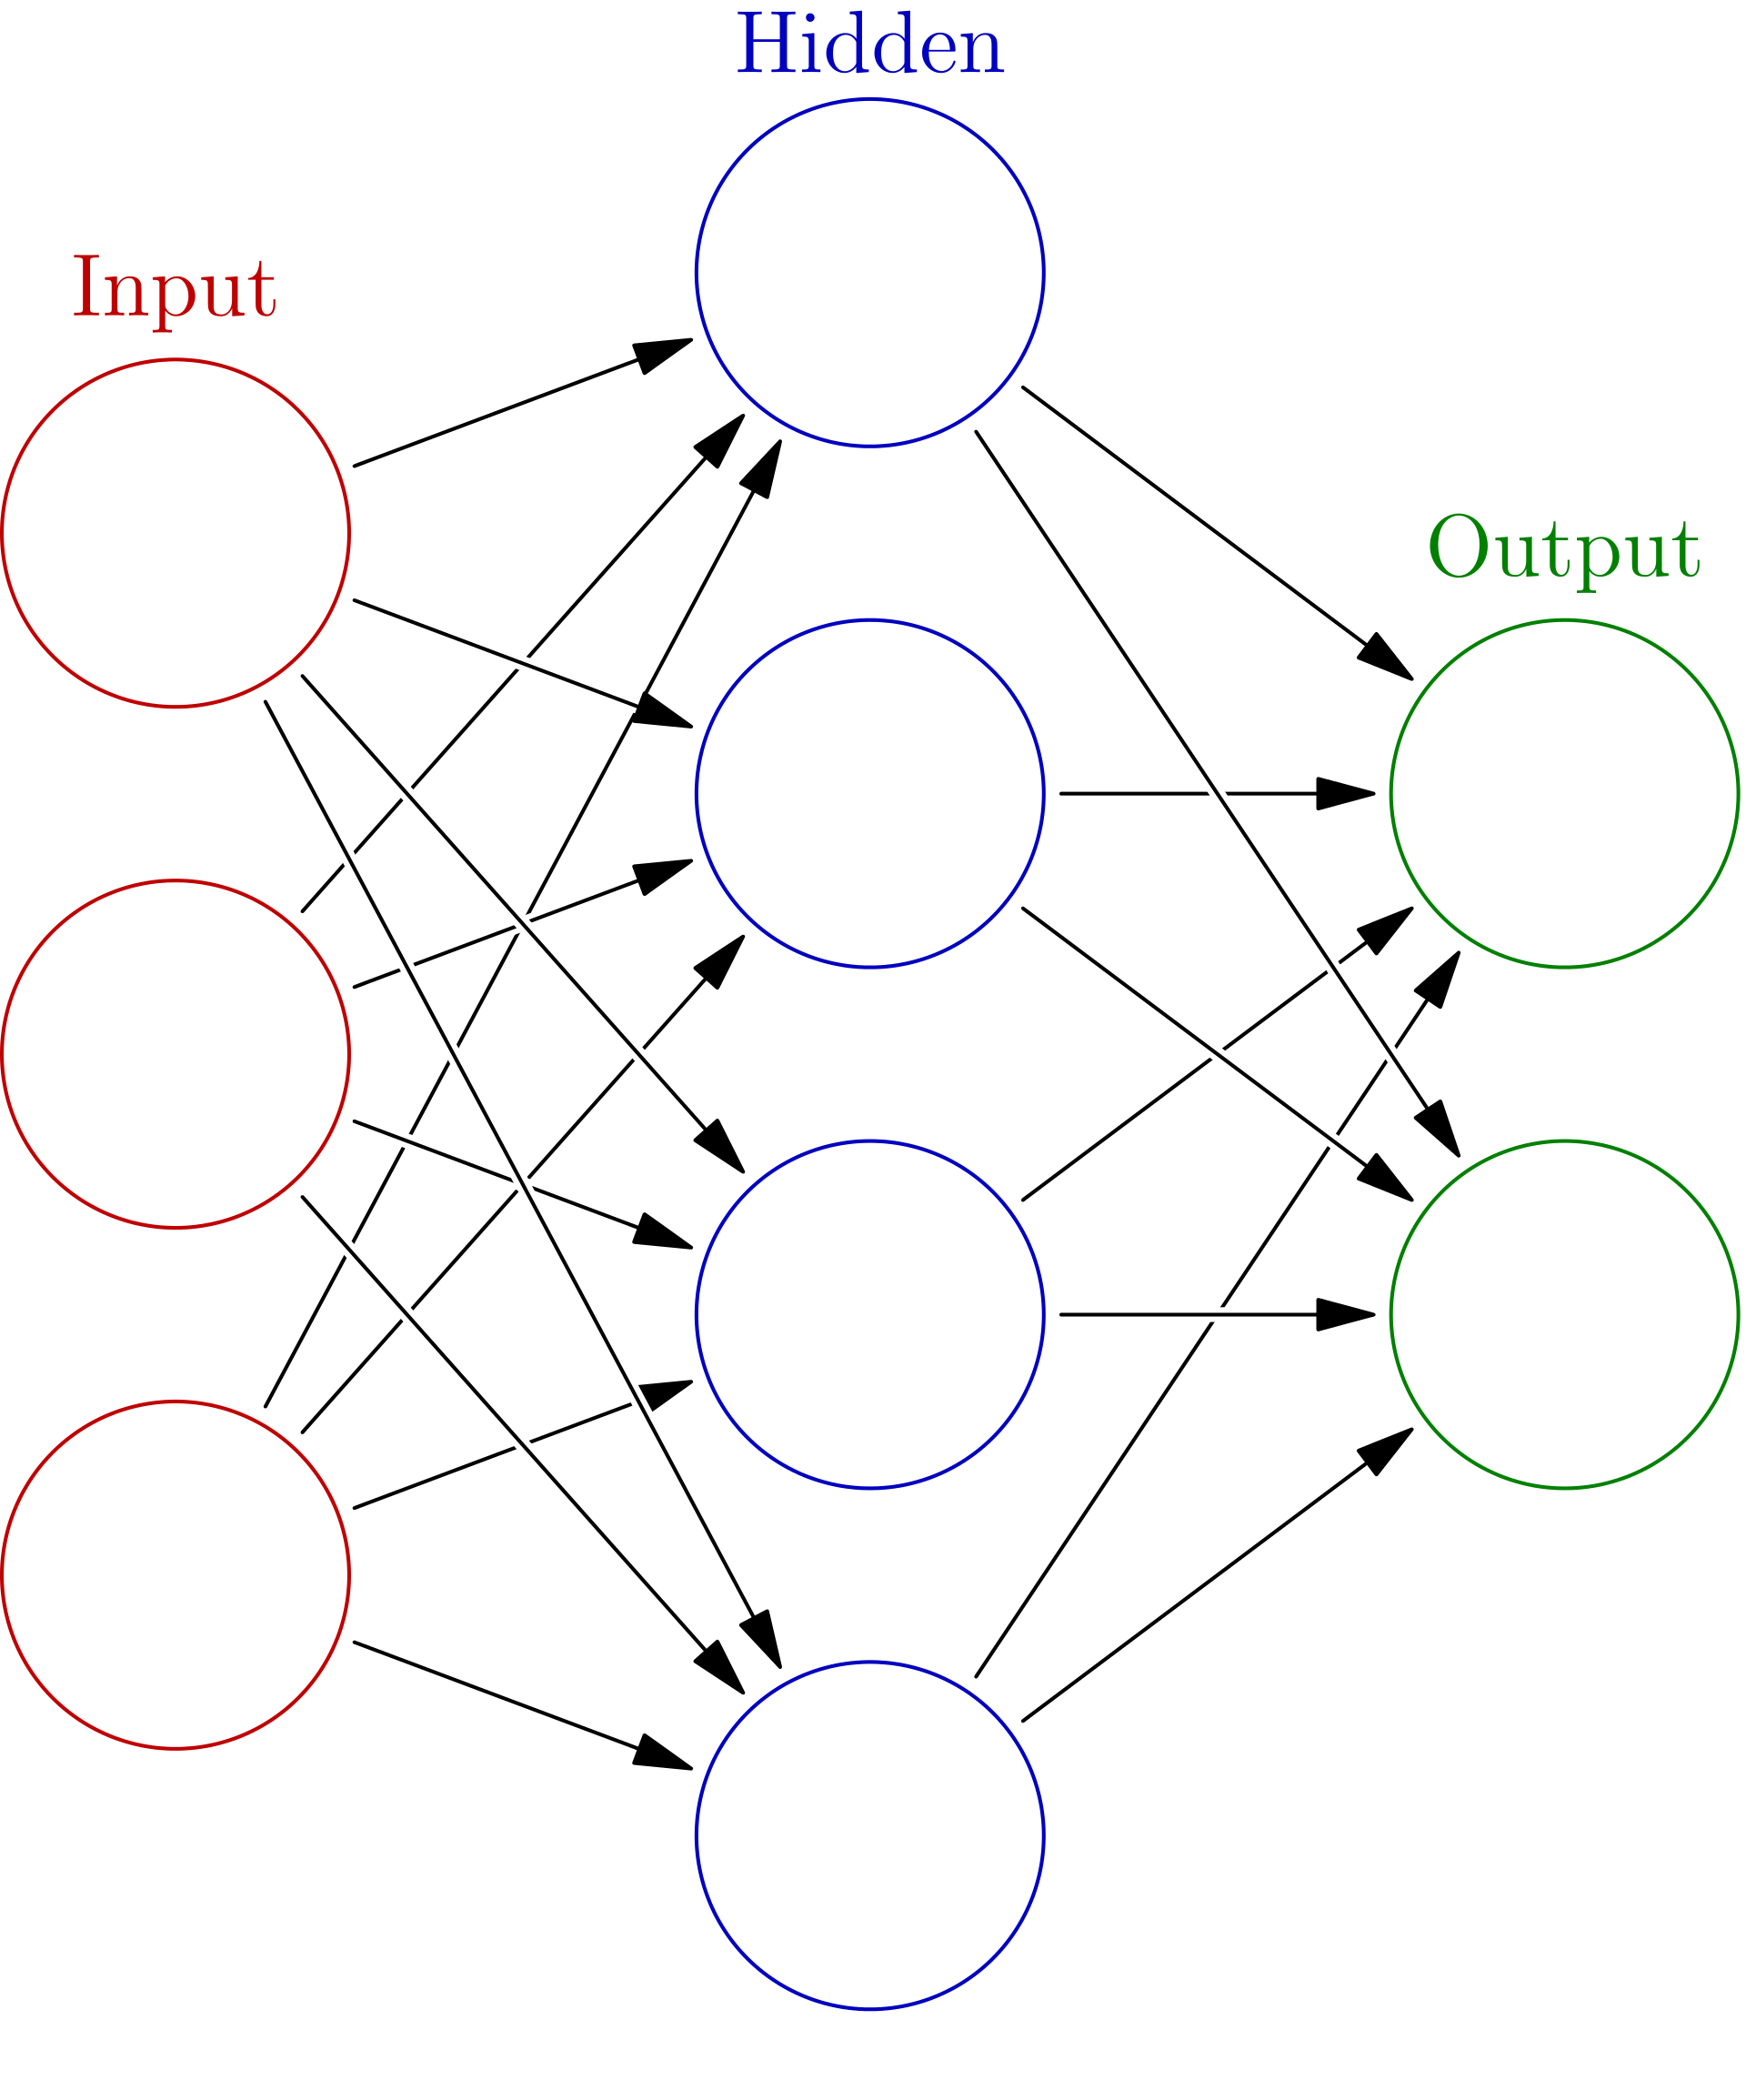
\includegraphics[scale=0.075]{Colored_neural_network.png}
\label{simplenetwork}
\end{figure}




\subsection{Konwolucyjne sieci neuronowe}{Sztuczne sieci neuronowe dominowały w początkowych latach badań, jednak wraz z rozwojem dziedziny opracowano inne modele sieci, które miały służyć już bardziej konkretnym zadaniom. Modelem, który został stworzony do analizowania scen wizualnych był model konwolucyjny, nazywany też splotowym. }
{Inspiracją do stworzenia tego modelu były odkrycia neurofizjologów Hubela i Wiesela z lat 50. i 60. zeszłego wieku. \cite{hubel1959receptive}\cite{hubel1963shape}\cite{hubel1968receptive} Odkryli oni, że neurony w korze wzrokowej reagują na określone pole widzenia. Każdy neuron ma swoje pole recepcyjne i reaguje na bodziec tylko w obrębie tego pola. Sieci konwolucyjne starają się odzworować sposób działania tych neuronów w korze wzrokowej. Zamiast patrzeć na obraz jako całość, każdy neuron jest odpowiedzialny za jego małą część. Neurony posiadająca pole recepcyjne nazywa się kernalami, albo filtrami, gdyż działają dokładnie jak klasyczne filtry, a warstwę filtrów nazywa się warstwą konwolucyjną. Sieci konwolucyjne składają się zazwyczaj z wielu warstw konwolucyjnych, przeplatanych innymi warstwami (np. próbkującymi), a na ich końcach umieszcza się jedną lub kilka warst w pełni połączonych. Zadaniem tych warstw w pełni połączonych jest dokonanie klasyfikacji na podstawie wyjścia z ostatniej warsty konwolucyjnej. To właśnie wyjście z ostatniej warstwy konwolucyjnej nazywane jest wektorem cech głębokich. Poniżej zostanie dokonany dokładniejszy opis warstwy konwolucyjnej, jak i również kilku innych rodzajów warstw, które są powszechnie używane w sieciach neuronowych.}

\subsubsection{Warstwa konwolucyjna}
{Warstw konwolucyjna to zbiór kerneli (filtrów), zawierających parametry, które należy nauczyć. Kernele są zazwyczaj małych rozmiarów, mniejszych od rozmiaru obrazu wejściowego. Typowym rozmiarem kernela jest np. 3x3x3, który oznacza, że pokrywa on obszar 3 na 3 piksele, w kolorze (trzeci wymiar to kanały RGB). Filtr jest następnie przesuwany przez cały obraz wejściowy, i w każdej jego pozycji obliczany jest iloczyn skalarny między nim a danymi wejściowymi (Rys. \ref{conv1}). W wyniku tego działania otrzymujemy pewną macierz, która nazywa się mapą aktywacji danego kernela. Mapy aktywacji wszystkich filtrów z danej warstwy są nakładane na siebie i tworzą trójwymiarowa macierz, która jest podawana na wyjściu warstwy konwolucyjnej, co pokazano na rysunku \ref{conv2}.}

\begin{figure}[h!]
\centering
\begin{minipage}{.5\textwidth}
  \centering
 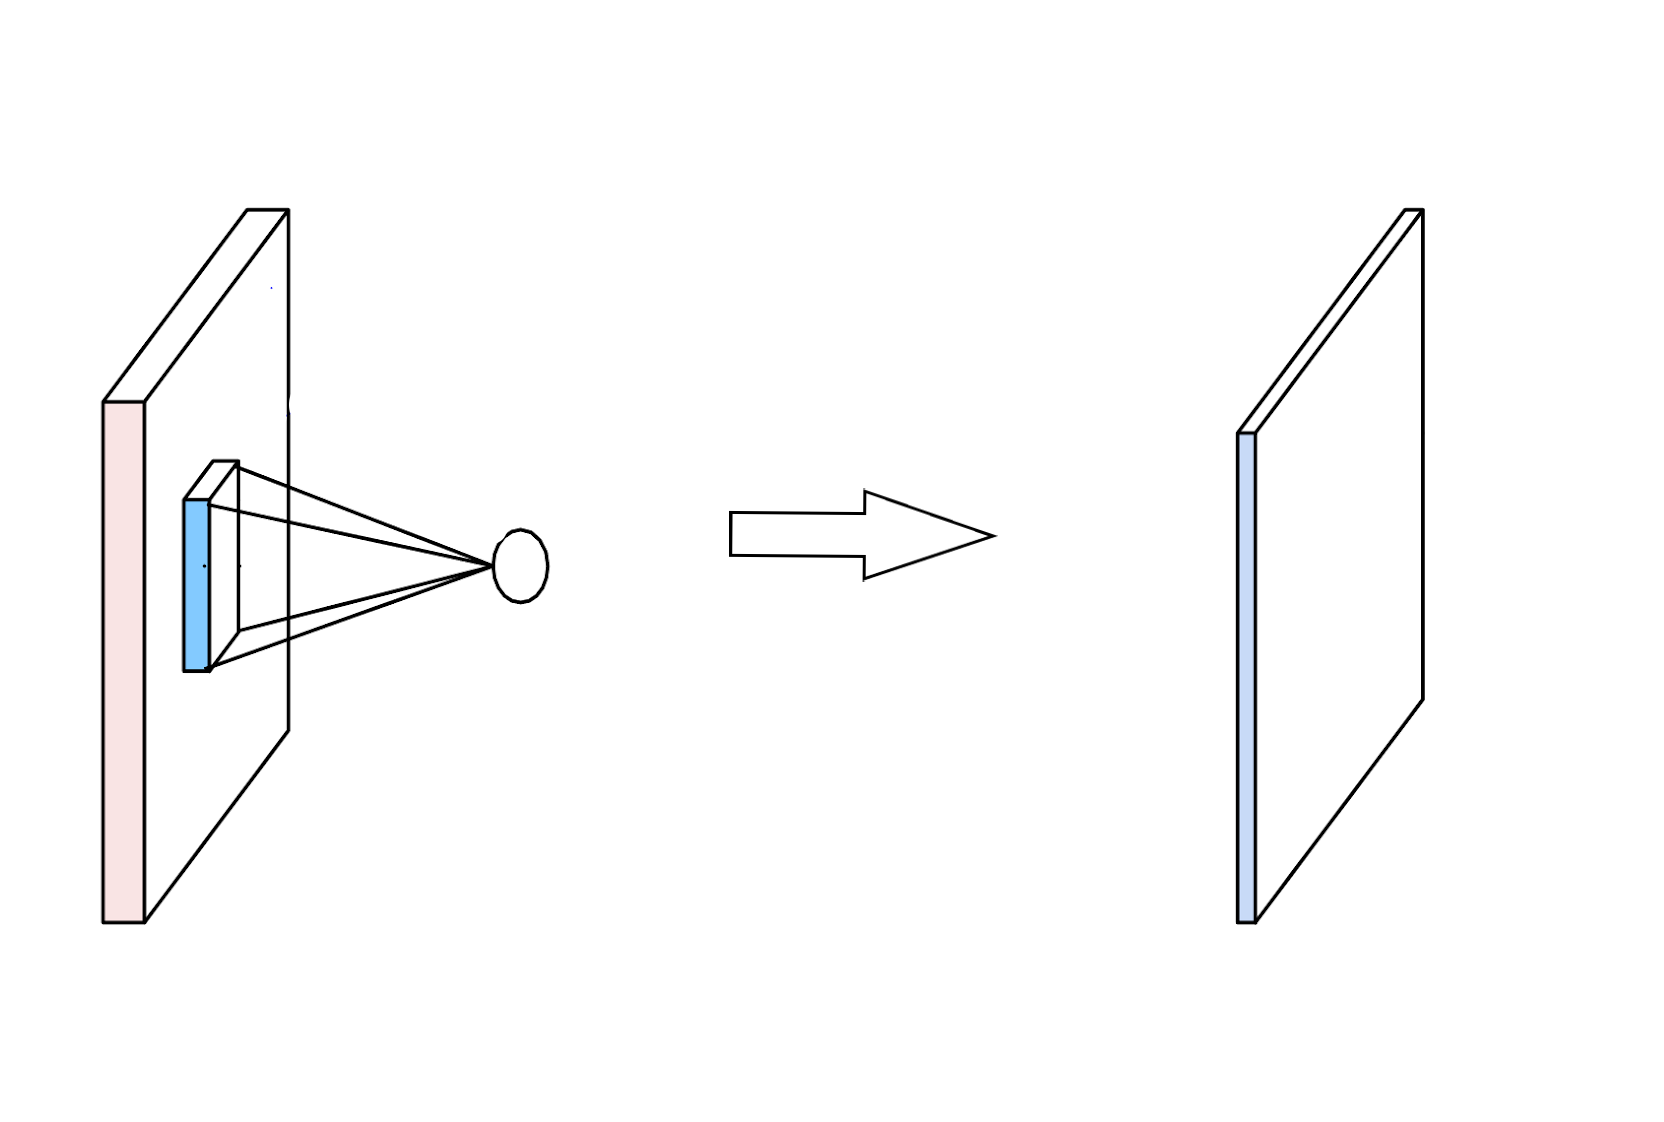
\includegraphics[scale=0.20,left]{conv1.png}
  \caption{Filtr o wymiarach 5x5x3}
\label{conv1}
\end{minipage}%
\begin{minipage}{.5\textwidth}
  \centering
  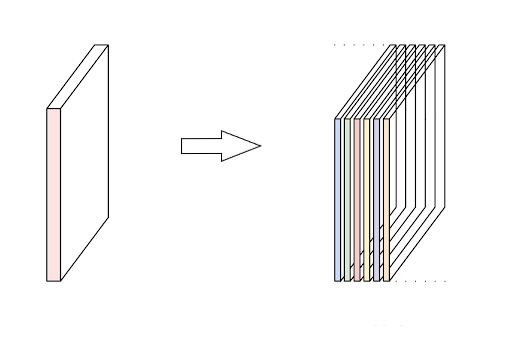
\includegraphics[scale=0.3,right]{conv2.png}
  \caption{Mapy aktywacji nakładane na siebie}
  \label{conv2}
\end{minipage}
\end{figure}






\subsubsection{Warstwa próbkująca}
{Nazywana też czasem warstwą łączenia, najcześciej umieszczana jest pomiędzy dwoma warstwami konwolucyjnymi. Jej zadaniem jest redukcja rozmiaru otrzymanych map aktywacji, co zmiejsza ilosć parametrów, których sieć musi się nauczyć. Ta warstwa opiera się u filtry najczęsciej o rozmiarach 2x2, które biorą maksymalną lub średnią wartość z każdego rejonu (rys. \ref{pool1}) i zmniejszają w ten sposób wysokość oraz szerokość danych, nie zmieniając jednak głębokości.}

\begin{figure}[h!]
\caption{Max pooling}

\centering
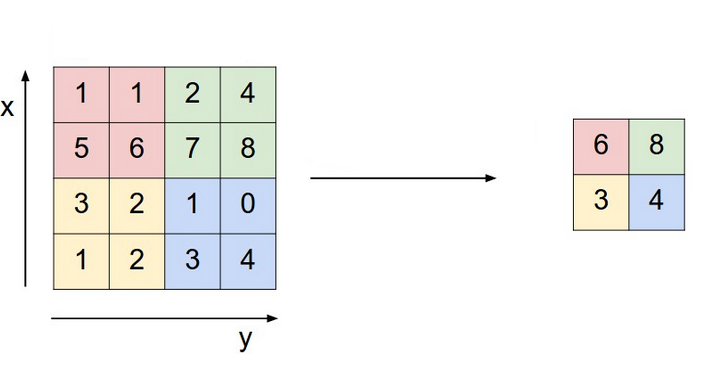
\includegraphics[scale=0.7]{pool1.png}
\label{pool1}
\end{figure}

\subsubsection{Warstwa aktywacyjne}
{Ta warstwa to funkcja matematyczna, która decyduje o tym, czy neuron ma być aktywny, czy nie, na podstawie jego wartości. Powinna być to funkcja szybka do obliczenia, bo będzie wykonywana dla każdego nueronu w sieci. Początkowo często używaną funkcją był $\tanh(x)$ (rys. \ref {tanh}) , ale z czasem okazało się że fukncja rektyfikowanej jednostki liniowej (ReLu), definiowanej jako $\max(0,x)$(rys. \ref{ReLu}) pozwala osiagnąć lepsze wyniki \cite{nair2010rectified}\cite{glorot2011deep} i aktualnie jest najczęściej używaną funkcją aktywacji \cite{ramachandran2017searching}.}


\begin{figure}[h!]
\begin{minipage}{.5\textwidth}
  \centering
\begin{tikzpicture} [domain=-1.0:1.0]
\begin{axis}[
    y tick label style={
        /pgf/number format/.cd,
            fixed,   % po zakomentowaniu os rzednych jest indeksowana wykladniczo
            fixed zerofill, % 1.0 zamiast 1
            precision=1,
        /tikz/.cd
    },
    x tick label style={
        /pgf/number format/.cd,
            fixed,
            fixed zerofill,
            precision=2,
        /tikz/.cd
    }
]

\addplot [draw=red]{max(0,x)};
\end{axis} 
\end{tikzpicture}
\caption{ReLu.}
\label{ReLu}
\end{minipage}%
%\end{figure}
\begin{minipage}{.5\textwidth}
%\begin{figure}[h!]
\centering
\begin{tikzpicture} [domain=-1.0:1.0]
\begin{axis}[
    y tick label style={
        /pgf/number format/.cd,
            fixed,   % po zakomentowaniu os rzednych jest indeksowana wykladniczo
            fixed zerofill, % 1.0 zamiast 1
            precision=1,
        /tikz/.cd
    },
    x tick label style={
        /pgf/number format/.cd,
            fixed,
            fixed zerofill,
            precision=2,
        /tikz/.cd
    }
]

\addplot [draw=red]{tanh(\x)};
\end{axis} 
\end{tikzpicture}
\caption{Tangens hiperboliczny.}
\label{tanh}
\end{minipage}%
\end{figure}


\subsubsection{Warstwa normalizujące}
{Warstwa ta została zaproponowana w celu zmiejszenia złożoności obliczeniowej poprzez normalizację aktywacji neuronów \cite{ba2016layer}, jednak doświadczenia praktyczne sugerują, że ich wpływ jest znikomy, przez co stosowane są bardzo rzadko i tylko w kontretnych przypadkach.}

\subsubsection{Warstwa regularyzacji opuszczeń}
{Warstwa ta w sposób losowy wyłącza pewną część neuronów (najczęściej 50\%), poprzez ustawienie ich wartości na 0, co sprawia, że nie będą aktywne. Może wydawać się to nieintuicyjne, jednak ta technika sprawia, że sieć musi być bardziej elastyczna i nie może zawsze polegać na istniejących już połączeniach. Pozwala do zapobiegać nadmiernemu dopsowaniu sieci oraz sprawia, że sieć osiąga lepsze rezultaty\cite{srivastava2014dropout}\cite{dahl2013improving}\cite{hinton2012improving}.}

\subsection{Przykladowe modele sieci}
{Na przestrzeni lat pojawiło się kilka modeli sieci neuronowych, które, czy to ze względu na swoją innowacyjność, czy na uzyskiwane wyniki, miały wielki wpływ na rozwój dziedziny i są powszechnie znane w środowiskach naukowach.}
\subsubsection{LeNet\cite{lecun1998gradient}}
{Jest to pierwsza udana implementacja konwolucyjnej sieci neuronowej. Stworzona w latach 90. przez Yanna LeCuna służyła do rozpoznawania ręcznie pisanych cyfr z kodów pocztowych. Składała się z 3 warstw konwolucyjnych na przemian z warstwami próbkującymi, oraz z jednej warstwy w pełni połączonej na samym końcu, co pokazano na rysunku \ref{LeNet}. }

\begin{figure}[h]
\caption{Architektura sieci LeNet}

\centering
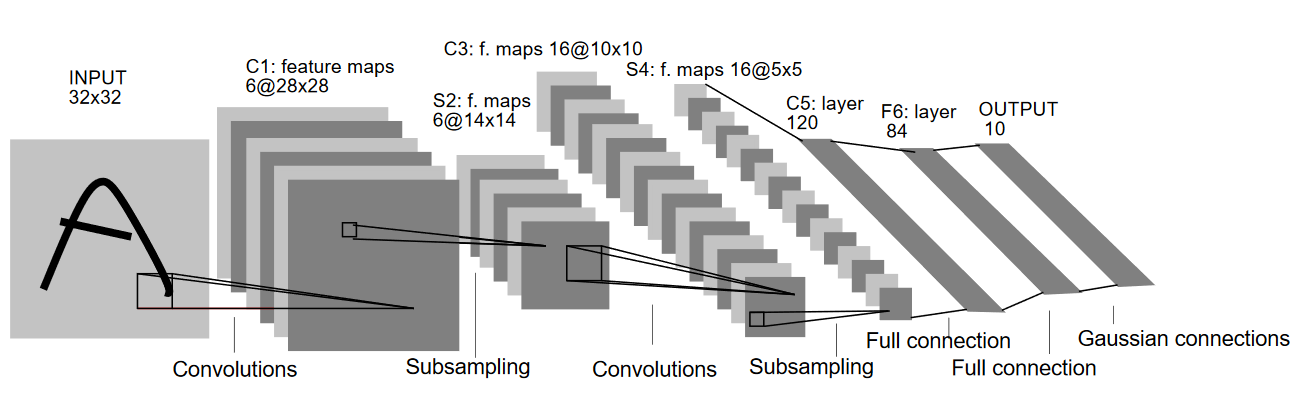
\includegraphics[scale=0.6]{le-net-5.png}
\label{LeNet}
\end{figure}

\subsubsection{AlexNet\cite{krizhevsky2012imagenet}}
{Sieci konwolucyjne zyskały popularność w latach 90., jednak wymagały dużej mocy obliczeniowej, które przy ówczesnym poziomie techniki były trudno dostępne (warto przypomnieć, że technologia CUDA powstała dopiero w 2007 roku), przez co wypadły z łask na rzecz maszyn wektorów wspierajacych\cite{girshick2014rich}. Sytuacja ta utrzymywała się aż to 2012 roku, kiedy to Alex Krizhevsky i in. stworzyli sieć AlexNet. Sieć osiągnęła najlepszy rezultat w konkursie ILSVRC, z błędem na poziomie 15,3\%, ponad 10 punktów procentowych lepiej od drugiego miejsca. Ten świetny rezultat na nowo pobudził zainteresowanie technologią sieci konwolucyjnych, a sieć ta jest uważana za jedną z najbardziej wpływowych w dziedzinie wizji komputerowej. Używa ona ReLu jako funkcji aktywacji, co nie było standardem w tym czasie. Zastosowana została warstwa regularyzacji opuszczeń z prawdopodobieństwem 50\%, jak i również augmentacja danych, co zmniejszyło nadmierne dopasowanie, a użycie procesorów graficznych pozwoliło na szybsze wykonanie kosztownych obliczeń. Na rysunku \ref{AlexNet} pokazano architekturę sieci AlexNet.}
\begin{figure}[h]
\caption{Architektura sieci AlexNet. Sieć została tutaj podzielona na dwie równoległe części, ponieważ obliczenia były dzielone pomiędzy dwie jednostki graficzne.}

\centering
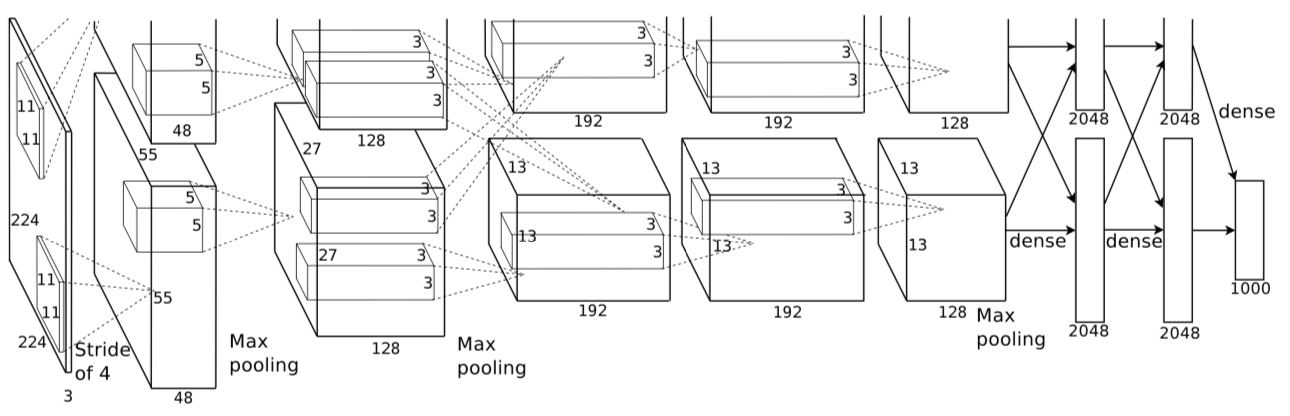
\includegraphics[scale=0.24]{alex.png}
\label{AlexNet}
\end{figure}

\subsubsection{VGG16\cite{simonyan2014very}}
\label{vg}
{Stworzona w 2014 roku przez Simonyana i Zissemana, pomimo tego, że zajęła 2 miejsce w konkursie ILSVRC, jest jedną z najbardziej rozpoznawalnych sieci w dziedzinie. Simonyan i Zisseman przyjęli inną strategi – zamiast zmieniać i testować różne wielkości warstw, użyli w niej warst konwolucyjnych o stałym wymiarze 3x3 oraz próbkujących o rozmiarze 2x2, a testowali jedynie różne głębokości sieci. W ramach pracy stworzono kilka wariantów sieci o różnej głębokości. Najlepszy okazał się wariant z 16 warstwami (rys. \ref{VGG}). Ten model pokazał, że głębokość sieci jest kluczowym czynnikiem decydującym o dobrym rezultacie.}
\begin{figure}[h!]
\caption{Architektura sieci VGG}

\centering
\includegraphics[scale=0.4]{VGG.png}
\label{VGG}
\end{figure}







\subsubsection{ResNet\cite{he2016deep}}
\label{Res}
{Sieć ta stworzona została przez Kaiminga He i in. i wygrała konkurs ILSVRC w 2015 roku. Jest przykładem sieci szczątkowej, w której niektóre połącznia pomiędzy warstwami są pomijane. Takie rozwiązanie pozwala na lepszą skalowalość wraz ze zwiększaniem liczby warstw oraz eliminuje problem tzw. zanikającego gradientu. Sieć ta posiada olbrzymią liczbę 152 warstw, i ta glebokość w połączeniu z nową technologią sprawiła, że przez długi czas była ona szczytowym osiągnięciem technologii.}

\section{R-CNN}
{Zastosowanie konwolucyjnych sieci neuronowych w problemie klasyfikacji jest stosunkowo proste, ponieważ wymiary danych wejściowych oraz wyjściowych są stałe. W przypadku detekcji jednak pojawia się problem, ponieważ liczba obiektów na zdjęciach może być różna, więc nasza sieć musiałaby dawać wyniki o zmiennych rozmiarach, co jest sprzeczne z jej zasadą działania. Początkowym rozwiązaniem było użycie okna, które przesuwało się po obrazie w każdej pozycji oraz klasyfikowało zaznaczony obszar \cite{szegedy2013deep}. Okno musiało sprawdzić każdą możliwą lokalizację, dodatkowo musiało zmieniać rozmiar, co skutkowało ogromną ilością obliczeń.}

{W celu rozwiązania tego problemu Ross Girshick i in. zaproponowali w 2014 roku rozwiązanie – regionalną konwolucyjną sieć neuronową\cite{girshick2014rich}. Rozwiązanie to zakłada, że najpierw z obrazu wydzielamy propozycje około 2000 regionów, w których jest duże prawdopodobieństwo, że znajduje się jakiś obiekt. Do wydzielania tych regionów, nazywanych też regionami zainteresowań (\ang {RoI - Regions of Interest}), służy algorytm selektywnej selekcji, opisany dokładniej w podrozdziale \ref{ss}. Następnie każdy z tych regionów służy jako dane wejściowe do konwolucyjnej sieci neuronowej, która wyznacza dla niego wektor cech głębokich. Następnie te wektory poddawane są klasyfikacji. W pierwotnej wersji klasyfikacja ta była przeprowadzana za pomocą maszyny wektorów wspierających, ale można używać innych metod w celu poprawy dokładności sieci.}

{Podczas detekcji musimy zmierzyć się z jeszcze jednym zadaniem – musimy zlokalizować nasz obiekt na zdjeciu. Jako lokalizację przyjmuje się wyznaczenie prostokątu, w którym znajduje się obiekt. Pojawia się więc problem, w jaki sposób ocenić, czy wyznaczony przez nas obszar pokrywa się z prostokątem zawierającym obiekt. Nie możemy oczekiwać, że wyznaczymy dokładnie identyczny obszar, ponieważ byłoby to wręcz niemożliwe. Wystarczy nam, że nasz obszar tylko w pewnym stopniu będzie pokrywał prostokąt. W celu ewaluacji tej miary używa się operatora [IoU] (przecięcie nad połączeniem), który używa współczynnika matematycznego, zwanego indeksem Jaccarda, definiowanego jako: 

\begin{equation}
F(A,B) = \frac{| A \cap B|}{ |A \cup B|}\\
\end{equation}

Czyli iloraz cześci wspólnej oraz sumy obu obszarów. Próg, od którego uznajemy, że wyznaczony obszar zawiera obiekt jest wyznaczny umownie (zazwyczaj jest to 0.5), a jego zmiana może znacząco wpływać na wynik sieci \cite{girshick2014rich}. Obszary z miarą IoU powyżej tego progu są uznawane za próbki dodatnie, ponieważ znajdują się w nich jakieś obiekty, a poniżej tego progu – ujemne, czyli zawierające tło.}

\subsection{Algorytm wyszukiwania selektywnego}
\label{ss}
{Algorytm ten\cite{uijlings2013selective} ma za zadanie wyznaczyć propozycje regionów, które będą później używane do detekcji obiektów. Na początku algorytm dokonuje segmentuje obraz na podstawie intensywności pikseli, bazując na zaproponowanej przez Felzenszwalba i in. metodzie segmentacji z zastosowaniem teorii grafów \cite{felzenszwalb2004efficient}. Następnie obszary, które są do siebie podobne, są ze sobą łączone. Podobieństwo obszarów określa się na podstawie 4 cech: koloru, tekstury, rozmiaru i kształtu.}
\subsubsection{Podobieństwo koloru}
{Dla każdego regionu generowany jest histogram danego kanału barwy. Wszystkie kanały są następnie zestawiane razem w wektor o określonej długości n, a podobieństwo jest wyliczane według wzoru:
\begin{equation}
P_{koloru}(r_{i},r_{j})= \sum_{k=1}^{n} min(c_{i}^k,c_{j}^k)\\
\end{equation}
Gdzie $c_{i}^k, c_{i}^k$ są wartością k-tego przedziału histogramu dla regionów kolejno: $r_{i}$ i $r_{j}$.
}
\subsubsection{Podobieństwo tekstury}
{
Dla każdego kanału liczonych jest 8 pochodnych Gaussa przy $\sigma=1$. Na ich podstawie dla każdego regionu tworzony jest histogram, a podobieństwo tekstur jest liczone jako:
\begin{equation}
P_{tekstury}(r_{i},r_{j})= \sum_{k=1}^{n} min(t_{i}^k,t_{j}^k)\\
\end{equation}
Gdzie $t_{i}^k,  t_{i}^k$ są wartością k-tego przedziału histogramu dla regionów kolejno: $r_{i}$ i $r_{j}$.

}
\subsubsection{Podobieństwo rozmiaru}
{To podobieństwo ma zachęcać mniejsze regiony do łączenia się ze sobą, jednocześnie pozwala unikać sytuacji, w której jeden region wchłania wszystkie inne. Dla obrazu o rozmiarze w pikselach $size(im)$ jest ono liczone jako:
\begin{equation}
P_{rozmiaru}(r_{i},r_{j})= 1- \frac{size(r_{i})+size(r_{j})}{size(im)}\\
\end{equation}}
\subsubsection{Podobieństwo kształu}
{Określa jak bardzo dwa regiony do siebie pasują. Jest zdefiniowane jako:
\begin{equation}
P_{kształtu}(r_{i},r_{j})= 1- \frac{size(BB_{ij})- size(r_{i})+size(r_{j})}{size(im)}\\
\end{equation}
Gdzie $BB_{ij}$ jest obwiednią dookoła regionów $r_{i}$ i $r_{j}$.
}


{Końcowe podobieństwo można ozyskać ze wzoru:
\begin{equation}
P(r_{i},r_{j})= a_{1}P_{koloru}+a_{2}P_{tekstury}+a_{3}P_{rozmiaru}+a_{4}P_{kształtu}\\
\end{equation}
Gdzie $a_{i} \in  \{0,1\}$ określa, czy miara podobieństwa jest użyta.
}


\subsection{Wady modelu R-CNN}
{Pomimo swojej użyteczności, model R-CNN nie jest pozbawiony wad. Konieczność wykonania obliczeń dla każdego z 2000 regionów sprawia, że model działa bardzo wolno, przez co wytrenowanie go może zająć duże ilości czasu. Dodatkowo nie może znaleźć on zastosowania w sytuacjach czasu rzeczywistego (np. analiza obrazu z kamery), przetworzenie każdego obrazu zajmuje średnio 40 sekund. Należy też zauważyć, że na etapie wyznaczania regionów nie następuje żadna nauka sieci  –  algorytm wyszukiwania selektywnego jest algorytmem stałym i niezależnym od parametrów sieci. Kolejne rozwiązania starają się rozwiązać te problemy. }
\section{Inne architektury}
\subsubsection{Fast R-CNN\cite{girshick2015fast}}
{Ross Girshick rok po publikacji swojej pracy opisującej R-CNN zaoproponował jej ulepszoną wersję – Fast R-CNN. Jak sama nazwa wskazuje, rozwiązanie to jest szybsze od swojej pierwszej wersji. Zamiast wyznaczać dużą liczbę regionów, na których następnie sięc dokonuje obliczeń, w tym modelu wrzucamy wejściowy obraz do sieci konwolucyjnej, a dopiero na otrzymanej z sieci mapie aktywacji dokonujemy podziału na regiony, które następnie klasyfikujemy. Dzięki temu rozwiązaniu znacząco zmniejszamy złożoność obliczeniową, co skutkuje 9-krotnym przyspieszeniem etapu treningu sieci oraz aż 213-krotnym przyspieszniem etapu testowania, przy jednoczesnym zwiększeniu precyzji sieci.}
\subsubsection{Faster R-CNN\cite{ren2015faster}}
{Wszystkie poprzednie metody używały algorytmu wyszukiwania selektywnego do wyznacznia propozycji regionów, jednak wraz ze wzrostem szybkości innych elementów modelu, ten algorytm stał się ,,wąskim gardłem'' obliczeniowym, dlatego postanowiono z niego zrezygnować. W ten sposób powstała architekura Faster R-CNN, jeszcze szybsza od swoich poprzedniczek, w której propozycje regionów są wyznaczane również przez równoległą sieć neuronową. Dzięki temu udało się jeszcze bardziej przyspieszyć działanie sieci, do poziomu 200 ms na obraz.}
\subsubsection{YOLO\cite{redmon2016you}}
{Architektura YOLO (\ang{You Only Look Once} – patrzy się tylko raz) stara się traktować problem detekcji jako problem regresji. Zamiast na cały obraz, sieć patrzy tylko na te fragmenty, w których jest bardziej prawdopodobne, że występuje jakiś obiekt. Wszystkie zadanie – lokalizację obiektów oraz klasyfikację wykonuje tylko jedna sieć, co drastycznie zwiększa szybkość tego rozwiązanie, pozwalając na zastosowanie go w celu detekcji w czasie rzeczywistym (z prędkością 45 klatek na sekundę). Wadą tego rozwiązania jest mniejsza precyzja sieci – często nie zauważa obiektów, szczególnie jeżeli są dość małe.}


 
\chapter{Wymagania i narzędzia}
{W tym rozdziale zostanie dokonany opis wymagań funkcjonalnych oraz niefunkcjonalnych pracy, oraz zaprezentowane zostaną diagramy przypadkow użycia. Następnia omówiona zostana użyte narzędzia oraz opisana zostania metodyka pracy nad projektowaniem i implenetacją.}
\section{Wymaganie funkcjonalne i niefunkcjonalne}
\subsection{Wymagania funkcjonalne}
{Projekt powinien realizować następujące funkcjonalności:
\begin{itemize}
\item{Użytkownik powinien móc dokonać wyboru architektury sieci.}
 \item {Powinna istnieć możliwość łatwego dodania innych architektur sieci.}
 \item{W ramach architektury, użytkownik ma mieć możliwość wczytania swojego modelu z pliku, wyświetlenia listy dostępnych modeli oraz wyboru modelu sieci.}
  \item {Dla określonych danych wejściowych, program ma mieć możliwość zapisania cech głębokich ektrahowanych przez sieć, wraz z odpowiadającymi im etykietami. Poprzez cechy głębokie rozumie się ostatnią warstwę sieci konwolucyjnej, którą sieć oblicza przed dokonaniem klasyfikacji. }
  \item{Użytkownik ma mieć możliwość wyboru formatu, w którym zostaną zapisane (tekst lub hdf5).}
  \item{Powinna istnieć możliwość wyboru dowolnych danych wejściowych, zgodnych z formatem PASCAL VOC, i to na tych danych zostanie wykonana ekstrakcja.}
  \item{Powinna istnieć możliwość wybrania klas, dla których zostanie dokonana esktrakcja}
  \item{W ramach projektu zostanie zaimplementowana architektura R-CNN i będzie ona domyślnie używaną architekturą (jeżeli użytkownik nie wskaże innej).}
\end{itemize}}
\subsection{Wymagania niefunkcjonalne}
{}
\section{Diagram przypadków użycia}
{
\begin{figure}[h!]

\centering
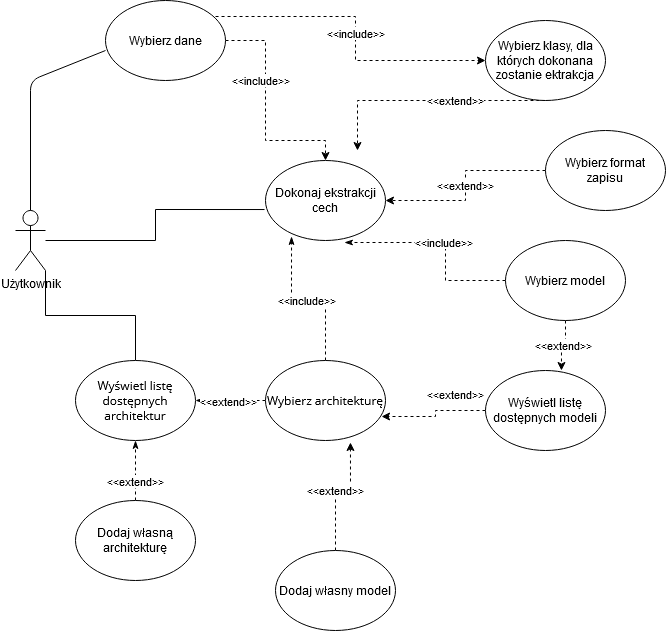
\includegraphics[scale=0.4]{usecase.png}
\caption{Diagram przypadków użycia}
\label{usecase}
\end{figure}

}
\section{Opis narzędzi}

\subsection{Python}
{Python jest językiem wysokopoziomowym językiem, który ze względu na swój rozbudowany system bibliotek oraz zwięzłą i przejrzystą składnię znajduje swoje zastosowanie w wielu dziedzinach, szczególnie tych związanych z uczeniem maszynowym. Python nie wymusza jednego paradygmatu programowania, jak np.C\#, lecz pozwala na użycie różnorodnych technik, takich jak programowanie obietkowe, programowanie strukturalne czy programowanie funkcyjne. Całość tworzonego narzędzia została stworzona właśnie w tym języku.}
\subsection{Keras i Tensorflow}
{Tensorflow to darmowa i otwartoźródłowa biblioteka, służąca głównie do rozwiązywania zadań z obszaru uczenia maszynowego. Keras słuzy jako to API \ang{Application Programming Interface} do biblioteki Tensorflow. Obie te biblioteki zostały użyte do implementacji konwolucyjnej sieci neuronowej. Oferują one możliwość wyborów modelów z już nauczonymi parametrami sieci (np. model VGG16, opisany w podrozdziale \ref{vg}, czy ResNet opisany w \ref{Res}).}
\subsection{Skimage i Imageio}
{Skimage oraz Imageio są blibliotekami języka python, które umożliwiają łatwe wczytywanie oraz przetwarzanie obrazów. W programie zostały one wykorzystane w implementacji algorytmu wyszukiwania selektywnego, jak i również do zmiany rozmiarów obrazu.}
\subsection{Abstract Base Classes}
{Abstract Base Classes (w skrócie – ABC) to moduł języka Python, który zapewnia infrastrukturę pozwalającą na zdefiniowanie klas abstrakcyjnych. Za jego pomocą tworzona jest abstrakcyjna klasa reprezentująca architekturę sieci. }
\subsection{Tkinter}
{Tkinter to biblioteka umożliwiajaca stworzenia GUI (ang. \ang{Graphical User Interface}) w Pythonie. Została użyta do stworzenia prostego interfejsu graficznego pomiędzy użytkownikiem a programem.}
\subsection{PASCAL VOC}
{W projekcie została wykorzystana baza danych PASCAL VOC 2012\cite{PASCAL} zawierająca 11530 obrazów z wyznaczonymi 27450 regionami zainteresowań, wraz z odpowiadającym im etykietami. Ta baza danych jest publicznie dostępna i przez lata była używana w ramach corocznego konkursu zzadać dotyczących wizji komputerowej.
}

\section{Metodyka pracy nad projektowaniem oraz implementcją}
{Pracę rozpoczęto od ogólnego zapoznania się z dziedziną oraz zrozumienia przedstawionego zagadnienia. Dzięki powszechnie dostępnym źródłom, takich jak artykuły internetowe oraz wykłady innych uczelni udostępniane na serwisach internetowych, szybko pojęto podstawy teoretyczne uczenia maszynowego oraz zasady działania konwolucyjnych sieci neuronowych.}

{Kolejnym krokiem było ustalenie wymagań projektu i wyznaczenie efektu końcowego. W celu lepszej wizualizacji wymagań stworzono również diagram przypadków użycia, ilustrujący przykładowe użycia systemu. Wymagania były następnie sukcesywnie  doprecyzowane, dzięki czemu przedstawiony problem stawał się łatwiejszy do zrozumienia.}

{Następnym krokiem była analiza źródeł odnoszących się już do głównego zagadnienia pracy. Dokonano jej poprzez lekturę publikacji naukowych oraz przeglądu znanych rozwiązań. Zapoznano się również w podobymi projektami dostępnymi publicznie i ich rozwiązaniami, dzięki czemu uzyskano lepszy punkt odniesienia. Następnie dokonano wyboru odpowiednich narzędzi oraz zapoznano się z ich dokumentacją techniczną.}
{Posiadając tą wiedzę teoretyczną, jasno przedstawiony cel oraz znajomość wybranych narzędzi, przystąpiono do implementacji projektu. Stworzono podstawowy model, do którego następnie dodawane były kolejne funkcjonalości, aż do osiągnięcia wyznaczonego efektu końcowego.}







\chapter{Specyfikacja zewnętrzna}
\begin{itemize}
\item  wymagania sprzętowe i programowe
\item  sposób instalacji
\item  sposób aktywacji
\item  kategorie użytkowników
\item  sposób obsługi
\item   administracja systemem
\item  kwestie bezpieczeństwa
\item  przykład działania
\item  scenariusze korzystania z systemu (ilustrowane zrzutami z ekranu lub generowanymi dokumentami)
\end{itemize}
 


\begin{figure}
\centering
\begin{tikzpicture}
\begin{axis}[
    y tick label style={
        /pgf/number format/.cd,
            fixed,   % po zakomentowaniu os rzednych jest indeksowana wykladniczo
            fixed zerofill, % 1.0 zamiast 1
            precision=1,
        /tikz/.cd
    },
    x tick label style={
        /pgf/number format/.cd,
            fixed,
            fixed zerofill,
            precision=2,
        /tikz/.cd
    }
]
\addplot [domain=0.0:0.1] {rnd};
\end{axis} 
\end{tikzpicture}
\caption{Podpis rysunku po rysunkiem.}
\label{fig:2}
\end{figure}

 

\chapter{Specyfikacja wewnętrzna}


 
\begin{itemize}
\item przedstawienie idei
\item architektura systemu
\item opis struktur danych (i organizacji baz danych)
\item komponenty, moduły, biblioteki, przegląd ważniejszych klas (jeśli występują)
\item przegląd ważniejszych algorytmów (jeśli występują)
\item szczegóły implementacji wybranych fragmentów, zastosowane wzorce projektowe
\item diagramy UML
\end{itemize}



Krótka wstawka kodu w linii tekstu jest możliwa, np. \lstinline|descriptor|, a nawet \lstinline|descriptor_gaussian|. 
Dłuższe fragmenty lepiej jest umieszczać jako rysunek, np. kod na rysunku \ref{fig:pseudokod}, a naprawdę długie fragmenty – w załączniku.

\begin{figure}
\centering
\begin{lstlisting}
class descriptor_gaussian : virtual public descriptor
{
   protected:
      /** core of the gaussian fuzzy set */
      double _mean;
      /** fuzzyfication of the gaussian fuzzy set */
      double _stddev;
      
   public:
      /** @param mean core of the set
          @param stddev standard deviation */
      descriptor_gaussian (double mean, double stddev);
      descriptor_gaussian (const descriptor_gaussian & w);
      virtual ~descriptor_gaussian();
      virtual descriptor * clone () const;
      
      /** The method elaborates membership to the gaussian fuzzy set. */
      virtual double getMembership (double x) const;
     
};
\end{lstlisting}
\caption{Klasa \lstinline|descriptor_gaussian|.}
\label{fig:pseudokod}
\end{figure}


\chapter{Weryfikacja i walidacja}
\begin{itemize}
\item sposób testowania w ramach pracy (np. odniesienie do modelu V)
\item organizacja eksperymentów
\item przypadki testowe zakres testowania (pełny/niepełny)
\item wykryte i usunięte błędy
\item opcjonalnie wyniki badań eksperymentalnych
\end{itemize}
 


\chapter{Podsumowanie i wnioski}
\begin{itemize}
\item uzyskane wyniki w świetle postawionych celów i zdefiniowanych wyżej wymagań
\item kierunki ewentualnych danych prac (rozbudowa funkcjonalna …)
\item problemy napotkane w trakcie pracy
\end{itemize}


\begin{table}
\centering
\caption{Opis tabeli nad nią.}
\label{id:tab:wyniki}
\begin{tabular}{rrrrrrrr}
\toprule
	         &                                     \multicolumn{7}{c}{metoda}                                      \\
	         \cmidrule{2-8}
	         &         &         &        \multicolumn{3}{c}{alg. 3}        & \multicolumn{2}{c}{alg. 4, $\gamma = 2$} \\
	         \cmidrule(r){4-6}\cmidrule(r){7-8}
	$\zeta$ &     alg. 1 &   alg. 2 & $\alpha= 1.5$ & $\alpha= 2$ & $\alpha= 3$ &   $\beta = 0.1$  &   $\beta = -0.1$ \\
\midrule
	       0 &  8.3250 & 1.45305 &       7.5791 &    14.8517 &    20.0028 & 1.16396 &                       1.1365 \\
	       5 &  0.6111 & 2.27126 &       6.9952 &    13.8560 &    18.6064 & 1.18659 &                       1.1630 \\
	      10 & 11.6126 & 2.69218 &       6.2520 &    12.5202 &    16.8278 & 1.23180 &                       1.2045 \\
	      15 &  0.5665 & 2.95046 &       5.7753 &    11.4588 &    15.4837 & 1.25131 &                       1.2614 \\
	      20 & 15.8728 & 3.07225 &       5.3071 &    10.3935 &    13.8738 & 1.25307 &                       1.2217 \\
	      25 &  0.9791 & 3.19034 &       5.4575 &     9.9533 &    13.0721 & 1.27104 &                       1.2640 \\
	      30 &  2.0228 & 3.27474 &       5.7461 &     9.7164 &    12.2637 & 1.33404 &                       1.3209 \\
	      35 & 13.4210 & 3.36086 &       6.6735 &    10.0442 &    12.0270 & 1.35385 &                       1.3059 \\
	      40 & 13.2226 & 3.36420 &       7.7248 &    10.4495 &    12.0379 & 1.34919 &                       1.2768 \\
	      45 & 12.8445 & 3.47436 &       8.5539 &    10.8552 &    12.2773 & 1.42303 &                       1.4362 \\
	      50 & 12.9245 & 3.58228 &       9.2702 &    11.2183 &    12.3990 & 1.40922 &                       1.3724 \\
\bottomrule
\end{tabular}
\end{table}  
 
 

%%%%%%%%%%%%%%%%%%%%%%%%%%%%
\backmatter 
\stepcounter{stronyPozaNumeracja}
\pagenumbering{Roman}
\setcounter{page}{\value{stronyPozaNumeracja}}
\pagestyle{tylkoNumeryStron}
%%%%%%%%%%%%%%%%%%%%%%%%%%%%%
 
\bibliographystyle{ieeetr}
\bibliography{bibliografia}

%%%%%%%%%%%%%%%%%%%%%%%%%%%%%



\begin{appendices}
 

\chapter*{Spis skrótów i symboli}

\begin{description}
\item[RoI] Region zainteresowań  (ang. \ang{Region of Interest})
\item[IoU] Przecięcie nad połączeniem (ang. \ang{Intersection over Union})
\item[CUDA] \ang{Compute Unified Device Architecture}
\item[ILSVRC] TODO
\item[API] Interfejs Programowania Aplikacji(ang. \ang{Application Programming Interface})
\item[GUI] Graficzny Interfejs Użytkownika (ang. \ang{Graphical User Interface})
\item[DNA] kwas deoksyrybonukleinowy (ang. \ang{deoxyribonucleic acid})
\item[MVC] model -- widok -- kontroler (ang. \ang{model--view--controller}) 
\item[$N$] liczebność zbioru danych
\item[$\mu$] stopnień przyleżności do zbioru
\item[$\mathbb{E}$] zbiór krawędzi grafu
\item[$\mathcal{L}$] transformata Laplace'a 
\end{description}


\chapter*{Źródła}

Jeżeli w pracy konieczne jest umieszczenie długich fragmentów kodu źródłowego, należy je przenieść do załącznika.

\begin{lstlisting}
partition fcm_possibilistic::doPartition
                             (const dataset & ds)
{
   try
   {
      if (_nClusters < 1)
         throw std::string ("unknown number of clusters");
      if (_nIterations < 1 and _epsilon < 0)
         throw std::string ("You should set a maximal number of iteration or minimal difference -- epsilon.");
      if (_nIterations > 0 and _epsilon > 0)
         throw std::string ("Both number of iterations and minimal epsilon set -- you should set either number of iterations or minimal epsilon.");
   
      auto mX = ds.getMatrix();
      std::size_t nAttr = ds.getNumberOfAttributes();
      std::size_t nX    = ds.getNumberOfData();
      std::vector<std::vector<double>> mV;
      mU = std::vector<std::vector<double>> (_nClusters);
      for (auto & u : mU)
         u = std::vector<double> (nX);
      randomise(mU);
      normaliseByColumns(mU);
      calculateEtas(_nClusters, nX, ds);
      if (_nIterations > 0)
      {
         for (int iter = 0; iter < _nIterations; iter++)
         {
            mV = calculateClusterCentres(mU, mX);
            mU = modifyPartitionMatrix (mV, mX);
         }
      }
      else if (_epsilon > 0)
      {
         double frob;
         do 
         {
            mV = calculateClusterCentres(mU, mX);
            auto mUnew = modifyPartitionMatrix (mV, mX);
            
            frob = Frobenius_norm_of_difference (mU, mUnew);
            mU = mUnew;
         } while (frob > _epsilon);
      }
      mV = calculateClusterCentres(mU, mX);
      std::vector<std::vector<double>> mS = calculateClusterFuzzification(mU, mV, mX);
      
      partition part;
      for (int c = 0; c < _nClusters; c++)
      {
         cluster cl; 
         for (std::size_t a = 0; a < nAttr; a++)
         {
            descriptor_gaussian d (mV[c][a], mS[c][a]);
            cl.addDescriptor(d);
         }
         part.addCluster(cl);
      }
      return part;
   }
   catch (my_exception & ex)                                  
   {                                                       
      throw my_exception (__FILE__, __FUNCTION__, __LINE__, ex.what()); 
   }                                                          
   catch (std::exception & ex)                                 
   {                                                            
      throw my_exceptionn (__FILE__, __FUNCTION__, __LINE__, ex.what()); 
   }                                                            
   catch (std::string & ex)                                     
   {                                                            
      throw my_exception (__FILE__, __FUNCTION__, __LINE__, ex);        
   }                                                             
   catch (...)                                                   
   {                                                             
      throw my_exception (__FILE__, __FUNCTION__, __LINE__, "unknown expection");       
   }  
}
\end{lstlisting}
 

\chapter*{Zawartość dołączonej płyty}

Do pracy dołączona jest płyta CD z~następującą zawartością:
\begin{itemize}
\item praca (źródła \LaTeX owe i końcowa wersja w \texttt{pdf}),
\item źródła programu,
\item dane testowe.
\end{itemize}

\listoffigures
\listoftables
	
\end{appendices}


\end{document}


%% Finis coronat opus.